\documentclass[journal]{IEEEtran}

\usepackage{blindtext}
\usepackage{cite}
\usepackage{graphicx}
\usepackage{array}
\usepackage{color}
\usepackage{tabularx}
\usepackage{epsfig}
\usepackage{amsmath}
\usepackage{amssymb}
\usepackage{bm}
\usepackage{wasysym}
\usepackage{circuitikz}
\usepackage{float}
\usetikzlibrary{arrows,shapes,calc,positioning}

\newcommand{\myscope}[2]
{\draw[thick,rotate=#2] (#1) circle (12pt)
(#1) ++(-0.35,-0.1) --++ (0.3,0.3) --++ (0,-0.3) --++(0.3,0.3) --++(0,-0.3);}

\begin{document}

\title{CSCE 221 \\ Problem Set 3}

\author{Jacob~Purcell,~\IEEEmember{Texas~A\&M,~Student}}

\maketitle
\section{Problem 1:}
\subsection*{A:}

Described on the figures below are $O$ values next to their corresponding computations.
$Fragment_1$ is found to have the behavior of $O(N)$, $Fragment_1$ goes as $O(N^2)$, and finally 
$Fragment_1$ goes as $O(N^4)$. In each case, the separated $O$ values are considered against 
eachother as $N \rightarrow \infty$. Since the functions separated in the figures are 
connected linearly, as $N \rightarrow \infty$ the influence of smaller $O$ becomes 
negligible. 

$$ Fragment_1:~\boxed{O(N)} $$
$$ Fragment_2:~\boxed{O(N^2)} $$
$$ Fragment_3:~\boxed{O(N^4)} $$

\begin{figure}[h!]
	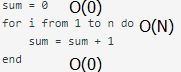
\includegraphics[scale = 1]{F1.PNG}
	\caption{$Fragment_1$}
\end{figure}

\begin{figure}[h!]
	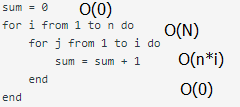
\includegraphics[scale = 1]{F2.PNG}
	\caption{$Fragment_1$}
\end{figure}

\begin{figure}[h!]
	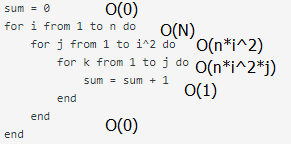
\includegraphics[scale = 1]{F3.PNG}
	\caption{$Fragment_1$}
\end{figure}

\subsection*{B:}

Code attached in separate document.

\subsection*{C:}

Figure 4. shows plotted output of the functions' recorded 
time growth with respect to the number of operations. The asymptotic trends in each fragment 
can be seen by dividing the times with their counterparts. As it turns out, the estimates 
approached a constant in separation for each recorded function. This was verified
by dividing several points along the curves, getting a similar constant every check.
As well, the constant would gradually approach what is to be construed
as the "true" proportionality constant. Following the form 

$$Fragment_n(N)~=~\gamma O(N),~\gamma~=~\frac{Fragment_n(N)}{O(N)}$$ 

where $\gamma$ is the constant of proportionality and $Fragment_n$ is the function of time, 
using $1000$ datapoints, $\gamma$ has been found to be:

$$ Fragment_1:~1 $$
$$ Fragment_2:~0.5005 $$
$$ Fragment_3:~Diverges $$

Running $Fragment_3$ to convergence proved difficult, and after 12 hours the following result was attained.
 $\gamma_{250} - \gamma_{240} = 1, \gamma_{377} - \gamma_{367} = 1$. This shows that the distance between proportionality
 constants every 10 iterations grows by 1. In order to show convergence, this difference must approach zero. Since $\gamma$ 
 diverges, $Fragment_3 > O(N^4)$. A guess was made and convergence was found when compared to $O(N^5)$. Upon further 
 investigation, a mistake in the initial estimation was found. Although "$i*j*k$" is correct, we must break the 
 iterators down into their corresponding factors of $N, i \rightarrow N, j \rightarrow i*i \rightarrow N^2, 
 k \rightarrow j \rightarrow N^2, \therefore i*j*k = N^5$, thus we find $\gamma$ of $Fragment_3$ to be $0.1005$.

$$ Fragment_1:~\boxed{O(N)} $$
$$ Fragment_2:~\boxed{O(N^2)} $$
$$ Fragment_3:~\boxed{O(N^5)} $$

 \begin{figure}[h!]
	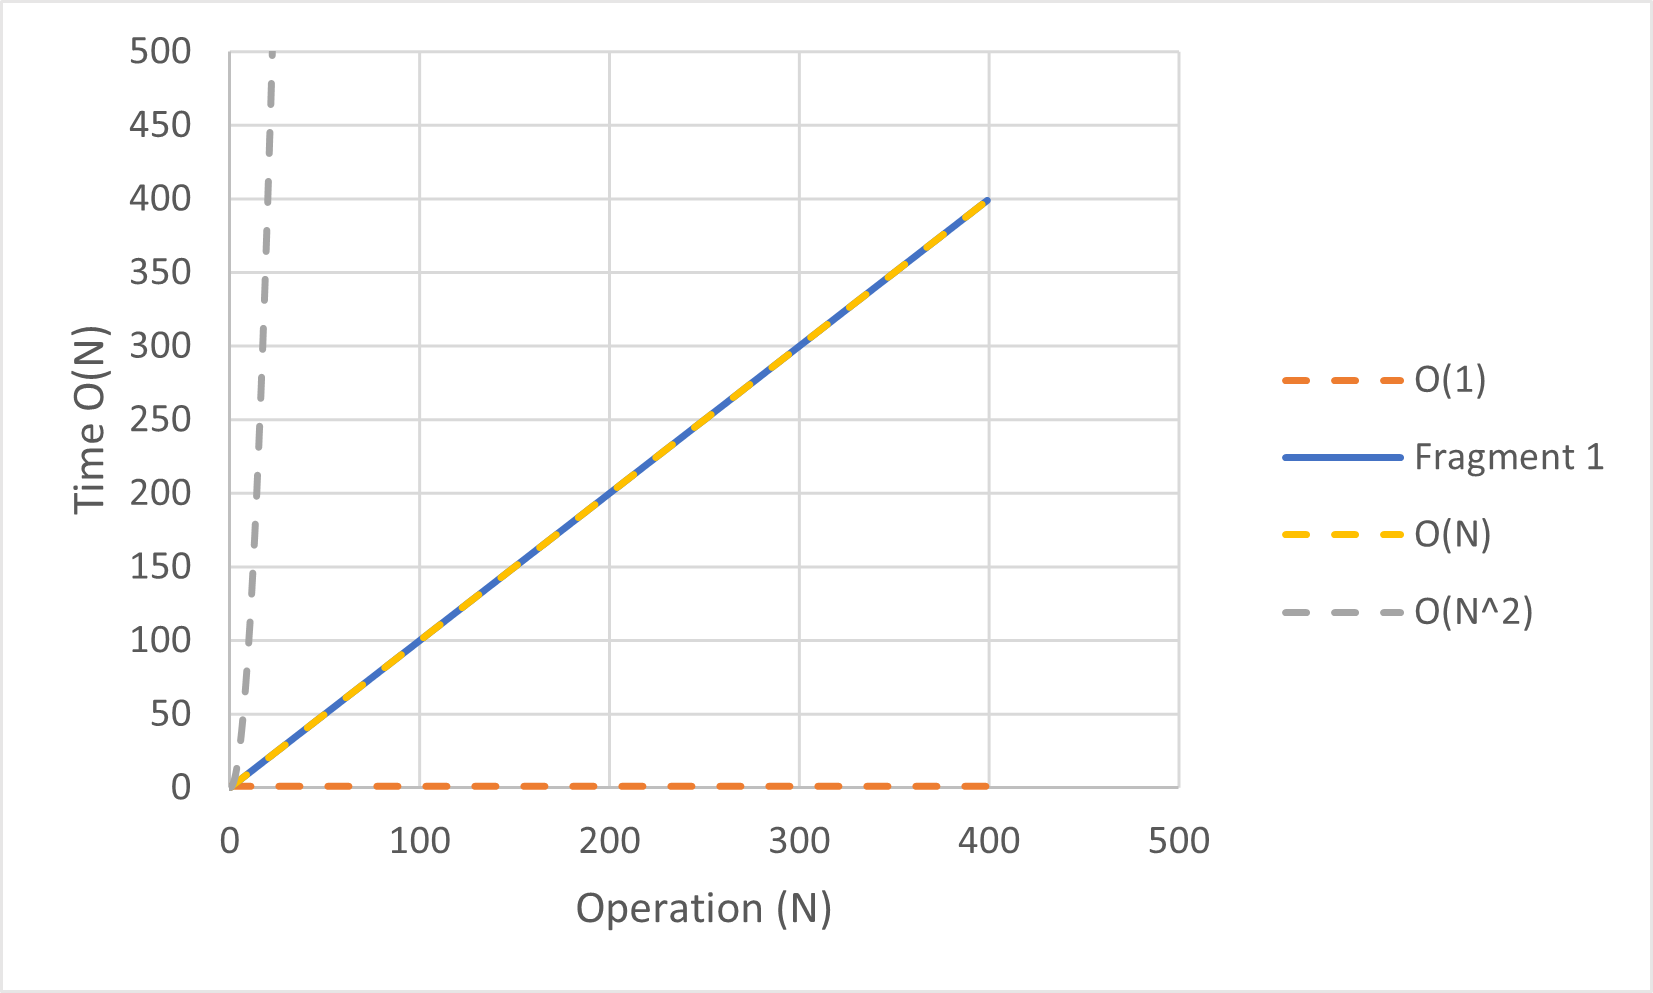
\includegraphics[scale = 0.7]{Picture1.PNG}
	\caption{$Fragment_1, O(N)$}
\end{figure}

\begin{figure}[h!]
	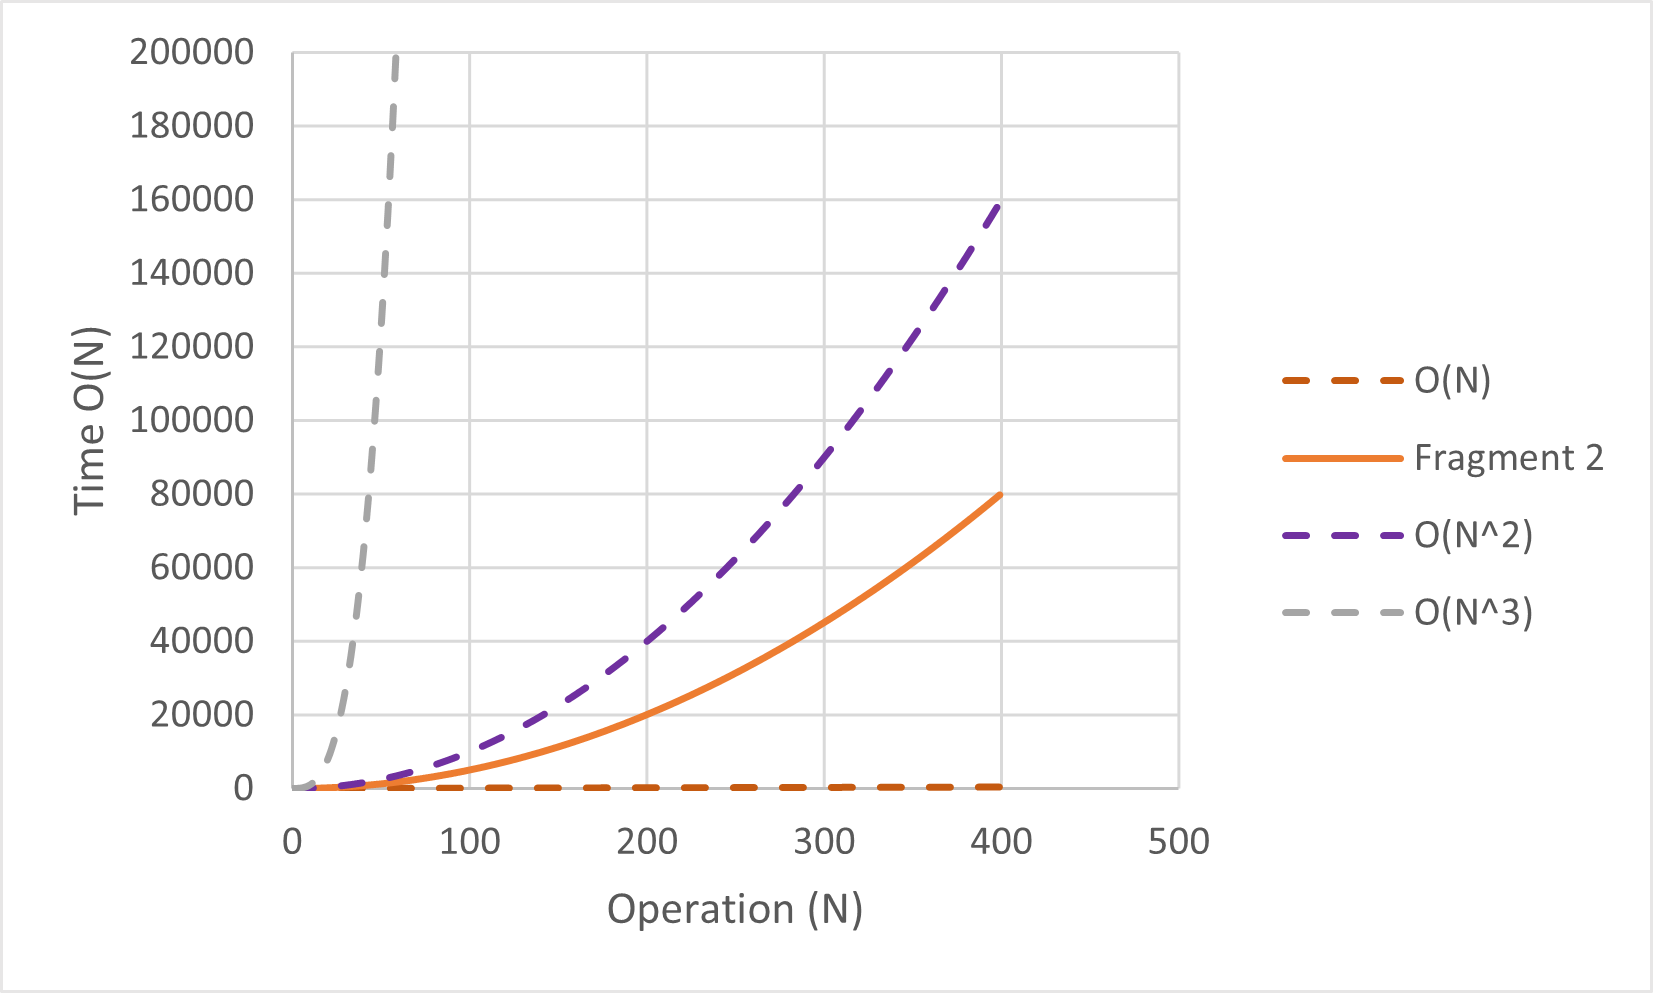
\includegraphics[scale = 0.7]{Picture2.PNG}
	\caption{$Fragment_2, O(N^2)$}
\end{figure}

\begin{figure}[h!]
	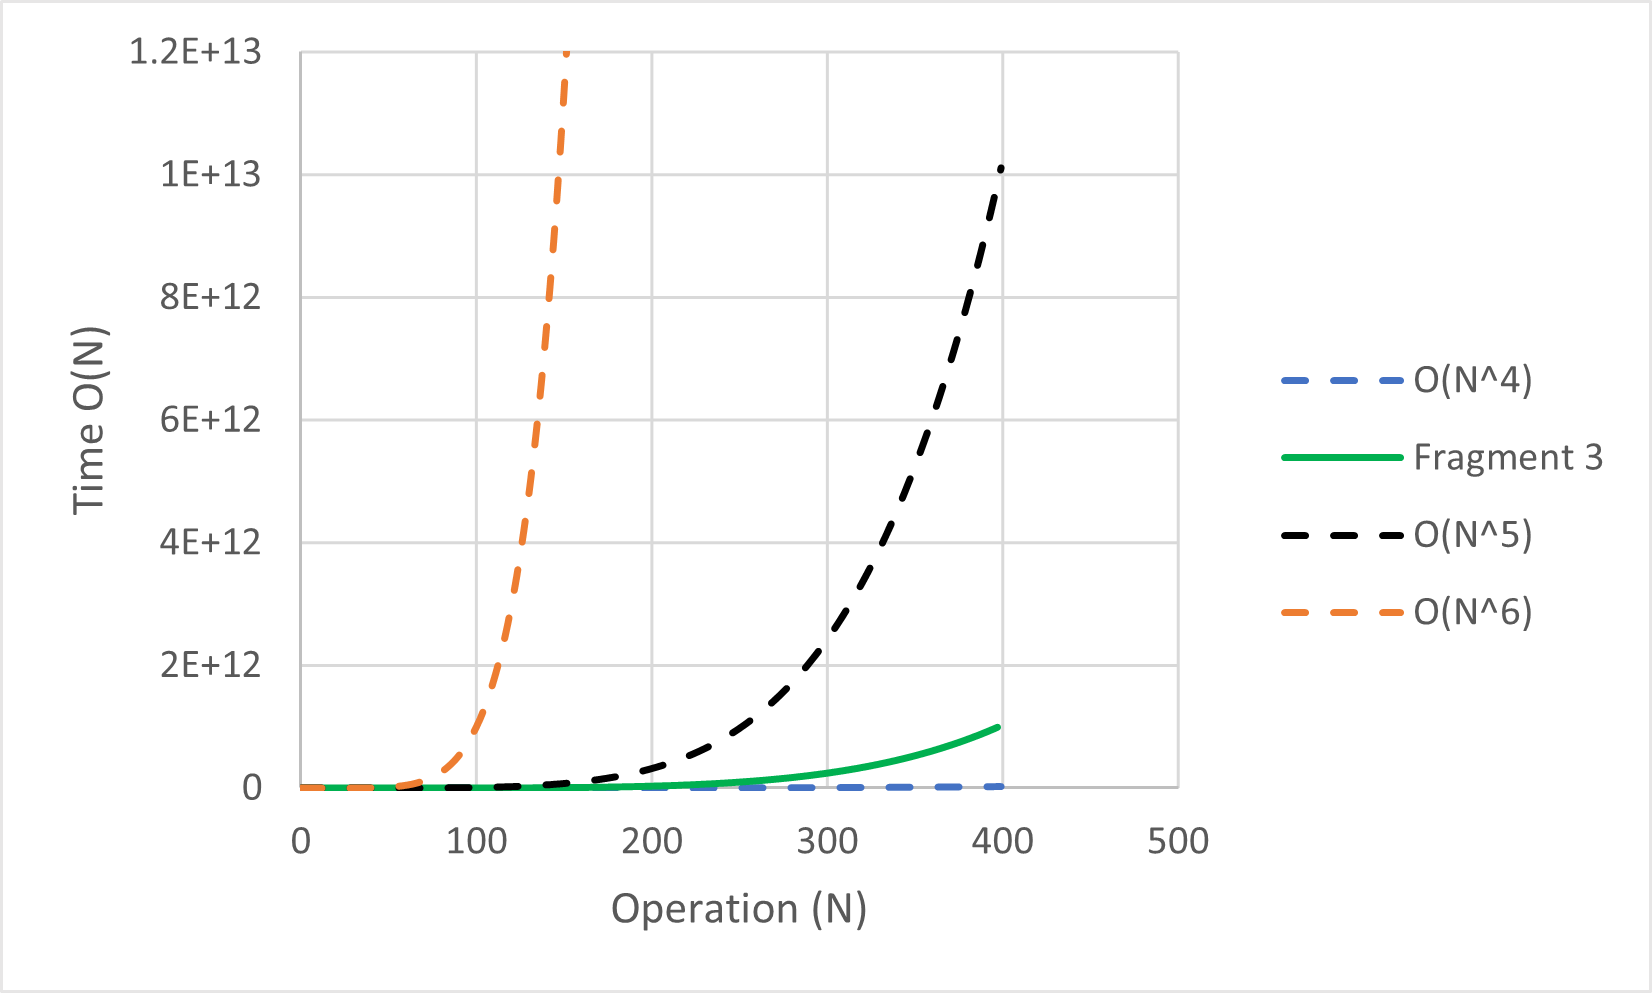
\includegraphics[scale = 0.7]{Picture3.PNG}
	\caption{$Fragment_3, O(N^5)$}
\end{figure}

\section{Problem 2:}

\subsection*{A:}
Psuedocode for hand calculations, A + B: \\
Since addition is commutative, the larger number will be called A. \\\\
For each digit in A that has a pair with B, $O(N)$\\
\indent add, $O(1)$ \\
\indent store first digit, $O(1)$ \\
\indent carry the 1 if present, $O(1)$\\
end \\\\

$\boxed{O(N)}$

\subsection*{B:}
Psuedocode for hand calculations, A * B:\\
Since multiplication is commutative, the larger number will be called A. \\\\
For each digit in A that has a pair with B, $O(N)$\\
\indent Multiply, $O(1)$\\
\indent store first digit, $O(1)$\\
\indent multiply the exess by number of zeroes in the B digit, $O(N)$\\
\indent add excess to next iteration, $O(1)$\\
end\\\\

$\boxed{O(N^2)}$

\subsection*{C:}
Psuedocode for hand calculations, A / B:\\\\
For each digit in A, $O(N)$ \\
\indent divide the front digit of A by the front digit in B, $O(1)$ \\
\indent store first digit (appended to rightmost end of number), $O(1)$\\
\indent store A \% B, $O(1)$ \\
\indent subtract A \% B from the next iteration, $O(1)$ \\
end\\\\

$\boxed{O(N)}$


\section{Problem 3:}

$$Given: f(x) = \Sigma_{i=0}^{N} a_i x^i$$ 

\subsection*{A:}
Naive exponentiation is estimated to be $\boxed{O(N^2)}$ since not only do summations grow with $N$, but $x^N$
takes $N$ multiplications to calculate. 

\subsection*{B:}
Fast exponentiation follows the system: 

$$X^N = X^{2^{\frac{N}{2}}}~for~even$$
$$X^N = X*X^{2{\frac{N-1}{2}}}~for~odd$$

Considering the even case, $X^{2^{2^{.^{.^{.^{\frac{N}{2^k}}}}}}}$. Requires $k$ 
operations ($O(k)$), which if we continue until $\frac{N}{2^k} = 1$, then 

$$N = 2^k$$
$$log_2 N = k$$

So, $O(k) \rightarrow O(\log_2 N)$, summed $N$ times, which makes $f(x)$ bounded by
$\boxed{O(N \log_2 N)}$.

\subsection*{C:}
Given function is estimated to be $O(N)$, since it computes 3 operations $N$ times.

\begin{figure}[h!]
	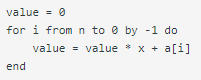
\includegraphics[scale = 1]{F4.PNG}
	\caption{}
\end{figure}

\section{Puzzle:}

Show that $X^{64}$ can be calculated in $8$ multiplications.

\begin{equation}
	X*X = X^2
\end{equation}

reusing $X^2$ and continuing the pattern leads to 

\begin{equation}
	X^2*X^2 = X^4
\end{equation}

\begin{equation}
	X^4*X^4 = X^8
\end{equation}

\begin{equation}
	X^8*X^8 = X^{16}
\end{equation}

\begin{equation}
	X^{16}*X^{16} = X^{32}
\end{equation}

\begin{equation}
	X^{32}*X^{32} = X^{64}
\end{equation}

6 multiplications using this method.




\end{document}
